\documentclass[11pt,a4paper]{ctexart}
\usepackage{common/ipara}

\definecolor{gold}{RGB}{218,165,32}
\tikzset{
  geom/.style={thick,draw=blue!80!black},
  aid/.style={thin,draw=gray!60},
  hline/.style={thick,draw=gold!90!black},
  vline/.style={thick,draw=teal,->,>=stealth},
  vpoint/.style={circle,fill=black,inner sep=1.2pt},
  centerpt/.style={circle,fill=gray!80,inner sep=1.2pt},
  moving/.style={circle,fill=gold!90!black,inner sep=1.5pt}
}

\newcommand{\vect}[1]{\overrightarrow{#1}}

% Truly scalene non-equilateral triangle ABC
\newcommand{\figGeneralCentroid}{%
\begin{tikzpicture}[scale=1.1,every node/.style={font=\small}]
  \coordinate (A) at (0.5, 3.0);
  \coordinate (B) at (-2.0, 0);
  \coordinate (C) at (2.5, 0);
  \coordinate (G) at (0.333, 1.0);
  
  \coordinate (D) at (-1.0, 1.2);
  \coordinate (E) at (2.0, 0.75);
  
  \draw[geom] (A)--(B)--(C)--cycle;
  \draw[aid,dashed] (A)--(0.25,0);
  \draw[hline,draw=gold!90!black,thick] (-1.6, 1.29)--(2.4, 0.69) node[right,font=\scriptsize,text=gold!90!black] {直线 \(l\)};
  
  \node[vpoint,label=above:$A$] at (A){};
  \node[vpoint,label=below left:$B$] at (B){};
  \node[vpoint,label=below right:$C$] at (C){};
  \node[centerpt,label=below left:$G$] at (G){};
  \node[moving,label=above left:$D$] at (D){};
  \node[moving,label=above right:$E$] at (E){};
\end{tikzpicture}}

% Solid Geometry Cone SO
\newcommand{\figCone}{%
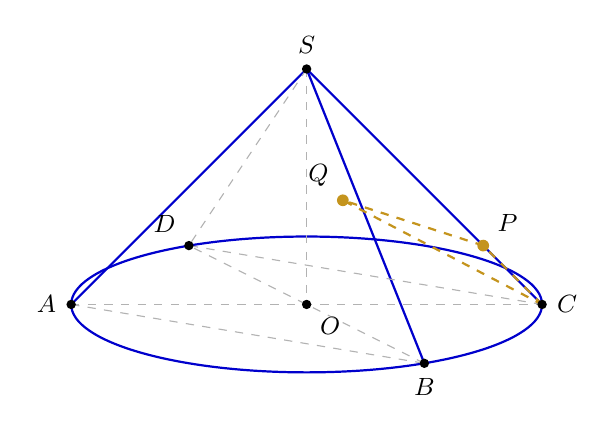
\begin{tikzpicture}[scale=1.15,every node/.style={font=\small}]
  % Base ellipse
  \draw[geom] (0,0) ellipse (2.6cm and 0.75cm);
  
  % Coordinates
  \coordinate (O) at (0,0);
  \coordinate (S) at (0,2.6);
  
  % Diameter AC along horizontal major axis (A left, C right)
  \coordinate (A) at (-2.6,0);
  \coordinate (C) at (2.6,0);
  
  % Diameter BD along tilted axis (D back-left, B front-right)
  \coordinate (D) at (-1.3,0.65);
  \coordinate (B) at (1.3,-0.65);
  
  % Points P and Q
  \coordinate (P) at (1.95,0.65); % 1/4 up from C on SC
  \coordinate (Q) at (0.4,1.15);   % Point in Plane SBD
  
  % Outermost generatrices (SA left, SC right)
  \draw[geom] (S)--(A);
  \draw[geom] (S)--(C);
  
  % Visible front generatrix
  \draw[geom] (S)--(B);
  
  % Hidden back generatrix & height
  \draw[aid,dashed] (S)--(D);
  \draw[aid,dashed] (S)--(O);
  
  % Base diameters & chords
  \draw[aid,dashed] (A)--(C);
  \draw[aid,dashed] (B)--(D);
  \draw[aid,dashed] (A)--(B);
  \draw[aid,dashed] (C)--(D);
  
  % Triangle CPQ
  \draw[hline,draw=gold!90!black,thick,dashed] (C)--(P)--(Q)--cycle;
  
  % Point labels with spacious offsets
  \node[vpoint,label=above:$S$] at (S){};
  \node[vpoint,label=below right:$O$] at (O){};
  \node[vpoint,label=left:$A$] at (A){};
  \node[vpoint,label=right:$C$] at (C){};
  \node[vpoint,label=below:$B$] at (B){};
  \node[vpoint,label=above left:$D$] at (D){};
  \node[moving,label=above right:$P$] at (P){};
  \node[moving,label=above left:$Q$] at (Q){};
\end{tikzpicture}}

% Standalone Isogonal Triangle for Question 8
\newcommand{\figIsogonalTriangle}{%
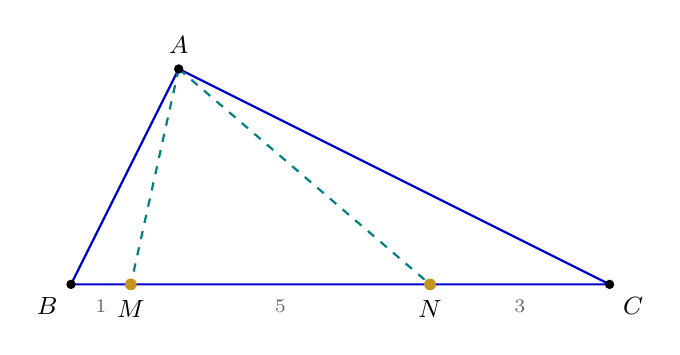
\begin{tikzpicture}[scale=0.95,every node/.style={font=\small}]
  \coordinate (B) at (0,0);
  \coordinate (M) at (0.8,0);
  \coordinate (N) at (4.8,0);
  \coordinate (C) at (7.2,0);
  \coordinate (A) at (1.44,2.88);
  
  \draw[geom] (A)--(B)--(C)--cycle;
  \draw[aid,dashed,thick,draw=teal] (A)--(M);
  \draw[aid,dashed,thick,draw=teal] (A)--(N);
  
  \node[vpoint,label=above:$A$] at (A){};
  \node[vpoint,label=below left:$B$] at (B){};
  \node[moving,label=below:$M$] at (M){};
  \node[moving,label=below:$N$] at (N){};
  \node[vpoint,label=below right:$C$] at (C){};
  
  % Length labels along BC
  \path (B) -- (M) node[midway,below=2pt,font=\scriptsize,text=gray!80!black] {$1$};
  \path (M) -- (N) node[midway,below=2pt,font=\scriptsize,text=gray!80!black] {$5$};
  \path (N) -- (C) node[midway,below=2pt,font=\scriptsize,text=gray!80!black] {$3$};
\end{tikzpicture}}

\begin{document}

\begin{center}
  {\Large\bfseries\sffamily 向量、函数与立体几何期末综合测试卷}
  \vspace{0.6em}
  
  {\small 考试时间：90 分钟 \qquad 满分：120 分（正卷 100 分 + 附加题 20 分） \qquad 姓名：\underline{\qquad\qquad} \qquad 成绩：\underline{\qquad\qquad}}
\end{center}

\vspace{1em}

\section*{一、 必答选择题（本大题共 3 小题，每小题 10 分，共 30 分。在每小题给出的四个选项中，只有一项是符合题目要求的）}

\vspace{0.8em}
\noindent\textbf{1.}（10 分）已知定义在 \(\mathbb{R}\) 上的奇函数 \(f(x)\) 满足 \(f(x) = f(x - 6)\)，且当 \(0 \le x \le 3\) 时，
\[
f(x) = \begin{cases} 
a + \log_{0.5}(x + 1), & 0 \le x \le 1,\\[0.3em]
(x - 2)(x - 3), & 1 < x \le 3
\end{cases} \quad (a \text{ 为常数})
\]
则 \(f(2010) + f(2011) + \cdots + f(2026)\) 的值为（\qquad）\\[0.6em]
A. \(-1\) \qquad\qquad\qquad B. \(0\) \qquad\qquad\qquad C. \(1\) \qquad\qquad\qquad D. \(-2\)

\vspace{1.5em}
\noindent\textbf{2.}（10 分）设函数 \(f(x) = \dfrac{2\sin x - 1}{\sin x + 2}\)，若 \([x]\) 表示不超过 \(x\) 的最大整数，记集合 \(M = \{y \in \mathbf{Z} \mid y = [f(x)], x \in \mathbf{R}\}\)，则 \(M =\)（\qquad）\\[0.6em]
A. \(\{-3, -2, -1, 0\}\) \qquad\qquad B. \(\{-3, -2, -1\}\) \qquad\qquad C. \(\{-2, -1, 0\}\) \qquad\qquad D. \(\{-3, -1, 0\}\)

\vspace{1.5em}
\noindent\textbf{3.}（10 分）已知 \(f\left(x+\dfrac{\pi}{3}\right)\) 是定义在 \(\mathbb{R}\) 上的奇函数，且 \(f(x)\) 仅有有限个零点，记其零点全集为 \(A = \{x_1, x_2, \cdots, x_n\}\)。若 \(|A| = 5\)，则 \(\cos\left(\sum_{x \in A} x\right) =\)（\qquad）\\[0.6em]
A. \(-1\) \qquad\qquad\qquad B. \(-\dfrac{1}{2}\) \qquad\qquad\qquad C. \(\dfrac{1}{2}\) \qquad\qquad\qquad D. \(1\)

\newpage

\section*{二、 必答解答题（本大题共 3 小题，共 70 分。解答应写出文字说明、证明过程或演算步骤）}

\vspace{1em}
\noindent\textbf{4.}（15 分）在 \(\triangle ABC\) 中，面积为 \(S\)，\(\angle BAC = \theta\)。已知 \(\vect{AB}\cdot\vect{AC} = 4\)，且 \(2 \le S \le 2\sqrt{3}\)。
求函数 \(f(\theta) = \sin 2\theta\) 的取值范围。

\vfill
\newpage

\noindent\textbf{5.}（25 分）如图，圆锥 \(SO\) 的顶点为 \(S\)，点 \(A, B, C, D\) 在底面圆 \(O\) 的圆周上，且 \(AC, BD\) 的交点为圆心 \(O\)，\(AB = 2\sqrt{2}\)，\(AC = 4\)，\(SO = 2\)。

\vspace{0.8em}
\begin{center}
  \figCone
\end{center}
\vspace{0.8em}

（1）求证：\(AC \perp BD\)，并求平面 \(SAB\) 与平面 \(SCD\) 夹角的余弦值；\\[0.8em]
（2）若 \(P\) 是母线 \(SC\) 上一点，且 \(CP = \dfrac{1}{4}CS\)，\(Q\) 是平面 \(SBD\) 内一点，求 \(\triangle CPQ\) 周长的最小值，并说明理由。

\vfill
\newpage

\noindent\textbf{6.}（30 分）在 \(\triangle ABC\) 中，点 \(G\) 是 \(\triangle ABC\) 的重心。过点 \(G\) 的直线 \(l\) 分别与线段 \(AB, AC\) 交于点 \(D, E\)（不同于端点）。设 \(\vect{AD} = \lambda\vect{AB}\)，\(\vect{AE} = \mu\vect{AC}\)（\(\lambda,\mu > 0\)）。

\vspace{0.8em}
\begin{center}
  \figGeneralCentroid
\end{center}
\vspace{0.8em}

（1）（8 分）求证：对于任意 \(\triangle ABC\)，均有 \(\dfrac{1}{\lambda} + \dfrac{1}{\mu} = 3\)；\\[0.8em]
（2）（10 分）求 \(\triangle ADE\) 与 \(\triangle ABC\) 的面积比 \(\dfrac{S_{\triangle ADE}}{S_{\triangle ABC}}\) 的取值范围；\\[0.8em]
（3）（12 分）若 \(\triangle ABC\) 为边长为 \(6\) 的等边三角形，当 \(\lambda = \dfrac{2}{3}\) 时，求 \(\dfrac{\tan\angle ABC}{\tan\angle ADC}\) 的值。

\vfill
\newpage

\section*{三、 附加拔高题（本大题共 2 小题，每小题 10 分，共 20 分。供学有余力者冲刺挑战）}

\vspace{1em}
\noindent\textbf{7.}（10 分，附加选择题）设 \(a \in \mathbf{R}\)，函数 
\[
f(x) = \begin{cases} 
\sin(2\pi x - 2\pi a), & x < a,\\[0.4em]
|x - a - 1| - 3a + 6, & x \ge a. 
\end{cases}
\]
记集合 \(A = \{x \in (0, +\infty) \mid f(x) = 0\}\)。则 “\(a \in \left(2, \dfrac{7}{3}\right]\)” 是 “集合 \(A\) 恰有 \(6\) 个元素” 的（\qquad）\\[0.6em]
A. 充分不必要条件 \qquad B. 必要不充分条件 \qquad C. 充要条件 \qquad D. 既不充分也不必要条件

\vspace{3em}
\noindent\textbf{8.}（10 分，附加解答题）如图，在 \(\triangle ABC\) 中，点 \(M, N\) 在边 \(BC\) 上，且点的顺序为 \(B-M-N-C\)，满足 \(BM = 1\)，\(MN = 5\)，\(NC = 3\)。若 \(\angle BAM = \angle CAN\)，求 \(\dfrac{AB}{AC}\) 的值。

\vspace{0.8em}
\begin{center}
  \figIsogonalTriangle
\end{center}

\vfill

\end{document}
